\documentclass[12pt,letterpaper]{article}
%\usepackage[utf8]{inputenc}
\UseRawInputEncoding
\usepackage[english]{babel}
\usepackage{listings}
\usepackage{xcolor}
\usepackage{graphicx}

%For syntax highlighting
\definecolor{codegreen}{rgb}{0,0.6,0}
\definecolor{codegray}{rgb}{0.5,0.5,0.5}
\definecolor{codepurple}{rgb}{0.58,0,0.82}
\definecolor{backcolour}{rgb}{1,1,1}

%%Sets different parameters
\lstdefinestyle{mystyle}{
    backgroundcolor=\color{backcolour},   
    commentstyle=\color{codegreen},
    keywordstyle=\color{magenta},
    numberstyle=\tiny\color{codegray},
    stringstyle=\color{codepurple},
    basicstyle=\ttfamily\footnotesize,
    breakatwhitespace=false,         
    breaklines=true,                 
    captionpos=b,                    
    keepspaces=true,                 
    numbers=left,                    
    numbersep=5pt,                  
    showspaces=false,                
    showstringspaces=false,
    showtabs=false,                  
    tabsize=4
}
\lstset{style=mystyle}

\title{\textbf{Department of Computer Science and Engineering}}
\author{\textbf{Shivanirudh S G, 185001146, Semester VII }}

\date{31 July 2021}

\begin{document}
\maketitle
\hrule
\section*{\center{UCS1712 - Graphics and Multimedia Lab}}
\hrule 
\bigskip\bigskip

%Assignment name
\subsection*{\center{\textbf{Exercise  4 : Midpoint Circle Drawing Algorithm in C++ using OpenGL}}}

%Objective
\subsection*{\flushleft{Objective:}}
\begin{flushleft}
     To plot points that make up the circle with center (xc,yc) and radius r using Midpoint circle drawing algorithm. Give atleast 2 test cases with centre as origin and elsewhere.   
\end{flushleft}

%Code
\subsection*{\flushleft{Code:}}
\begin{flushleft}
\lstinputlisting[language = C++]{Midpoint/Headers.h}
\lstinputlisting[language = C++]{Midpoint/Signatures.h}
\lstinputlisting[language = C++]{Midpoint/Helpers.h}
\lstinputlisting[language = C++]{Midpoint/main.cpp}
\end{flushleft}
\newpage
\subsection*{\flushleft{Output:}}
\textbf{Center at origin:}
\begin{figure}[h]
    \centering
    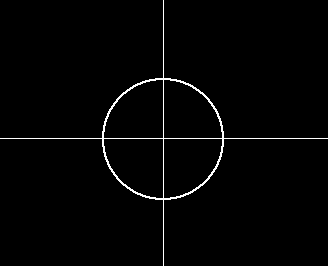
\includegraphics[height=7cm]{Midpoint/Outputs/Origin.png}
\end{figure}

\textbf{Choose center: (1 for origin, 2 for elsewhere): 1}\\
\textbf{Center:} (0, 0)
\textbf{Radius:} 60\\

\textbf{Points plotted}: 
(60, 0) (60, 1) (-60, 1) (60, -1) 
(-60, -1) (1, 60) (-1, 60) (1, -60) 
(-1, -60) (60, 2) (-60, 2) (60, -2) 
(-60, -2) (2, 60) (-2, 60) (2, -60) 
(-2, -60) (60, 3) (-60, 3) (60, -3) 
(-60, -3) (3, 60) (-3, 60) (3, -60) 
(-3, -60) (60, 4) (-60, 4) (60, -4) 
(-60, -4) (4, 60) (-4, 60) (4, -60) 
(-4, -60) (60, 5) (-60, 5) (60, -5) 
(-60, -5) (5, 60) (-5, 60) (5, -60) 
(-5, -60) (60, 6) (-60, 6) (60, -6) 
(-60, -6) (6, 60) (-6, 60) (6, -60) 
(-6, -60) (60, 7) (-60, 7) (60, -7) 
(-60, -7) (7, 60) (-7, 60) (7, -60) 
(-7, -60) (59, 8) (-59, 8) (59, -8) 
(-59, -8) (8, 59) (-8, 59) (8, -59) 
(-8, -59) (59, 9) (-59, 9) (59, -9) 
(-59, -9) (9, 59) (-9, 59) (9, -59) 
(-9, -59) (59, 10) (-59, 10) (59, -10) 
(-59, -10) (10, 59) (-10, 59) (10, -59) 
(-10, -59) (59, 11) (-59, 11) (59, -11) 
(-59, -11) (11, 59) (-11, 59) (11, -59) 
(-11, -59) (59, 12) (-59, 12) (59, -12) 
(-59, -12) (12, 59) (-12, 59) (12, -59) 
(-12, -59) (59, 13) (-59, 13) (59, -13) 
(-59, -13) (13, 59) (-13, 59) (13, -59) 
(-13, -59) (58, 14) (-58, 14) (58, -14) 
(-58, -14) (14, 58) (-14, 58) (14, -58) 
(-14, -58) (58, 15) (-58, 15) (58, -15) 
(-58, -15) (15, 58) (-15, 58) (15, -58) 
(-15, -58) (58, 16) (-58, 16) (58, -16) 
(-58, -16) (16, 58) (-16, 58) (16, -58) 
(-16, -58) (58, 17) (-58, 17) (58, -17) 
(-58, -17) (17, 58) (-17, 58) (17, -58) 
(-17, -58) (57, 18) (-57, 18) (57, -18) 
(-57, -18) (18, 57) (-18, 57) (18, -57) 
(-18, -57) (57, 19) (-57, 19) (57, -19) 
(-57, -19) (19, 57) (-19, 57) (19, -57) 
(-19, -57) (57, 20) (-57, 20) (57, -20) 
(-57, -20) (20, 57) (-20, 57) (20, -57) 
(-20, -57) (56, 21) (-56, 21) (56, -21) 
(-56, -21) (21, 56) (-21, 56) (21, -56) 
(-21, -56) (56, 22) (-56, 22) (56, -22) 
(-56, -22) (22, 56) (-22, 56) (22, -56) 
(-22, -56) (55, 23) (-55, 23) (55, -23) 
(-55, -23) (23, 55) (-23, 55) (23, -55) 
(-23, -55) (55, 24) (-55, 24) (55, -24) 
(-55, -24) (24, 55) (-24, 55) (24, -55) 
(-24, -55) (55, 25) (-55, 25) (55, -25) 
(-55, -25) (25, 55) (-25, 55) (25, -55) 
(-25, -55) (54, 26) (-54, 26) (54, -26) 
(-54, -26) (26, 54) (-26, 54) (26, -54) 
(-26, -54) (54, 27) (-54, 27) (54, -27) 
(-54, -27) (27, 54) (-27, 54) (27, -54) 
(-27, -54) (53, 28) (-53, 28) (53, -28) 
(-53, -28) (28, 53) (-28, 53) (28, -53) 
(-28, -53) (53, 29) (-53, 29) (53, -29) 
(-53, -29) (29, 53) (-29, 53) (29, -53) 
(-29, -53) (52, 30) (-52, 30) (52, -30) 
(-52, -30) (30, 52) (-30, 52) (30, -52) 
(-30, -52) (51, 31) (-51, 31) (51, -31) 
(-51, -31) (31, 51) (-31, 51) (31, -51) 
(-31, -51) (51, 32) (-51, 32) (51, -32) 
(-51, -32) (32, 51) (-32, 51) (32, -51) 
(-32, -51) (50, 33) (-50, 33) (50, -33) 
(-50, -33) (33, 50) (-33, 50) (33, -50) 
(-33, -50) (49, 34) (-49, 34) (49, -34) 
(-49, -34) (34, 49) (-34, 49) (34, -49) 
(-34, -49) (49, 35) (-49, 35) (49, -35) 
(-49, -35) (35, 49) (-35, 49) (35, -49) 
(-35, -49) (48, 36) (-48, 36) (48, -36) 
(-48, -36) (36, 48) (-36, 48) (36, -48) 
(-36, -48) (47, 37) (-47, 37) (47, -37) 
(-47, -37) (37, 47) (-37, 47) (37, -47) 
(-37, -47) (46, 38) (-46, 38) (46, -38) 
(-46, -38) (38, 46) (-38, 46) (38, -46) 
(-38, -46) (46, 39) (-46, 39) (46, -39) 
(-46, -39) (39, 46) (-39, 46) (39, -46) 
(-39, -46) (45, 40) (-45, 40) (45, -40) 
(-45, -40) (40, 45) (-40, 45) (40, -45) 
(-40, -45) (44, 41) (-44, 41) (44, -41) 
(-44, -41) (41, 44) (-41, 44) (41, -44) 
(-41, -44) (43, 42) (-43, 42) (43, -42) 
(-43, -42) (42, 43) (-42, 43) (42, -43) 
(-42, -43)

\newpage
\textbf{Center at (xc, yc):}
\begin{figure}[h]
    \centering
    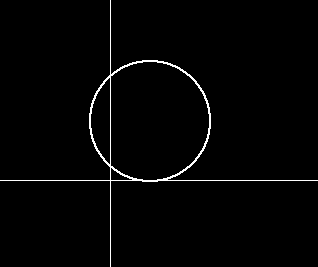
\includegraphics[height=7cm]{Midpoint/Outputs/Quadrant.png}
\end{figure}

\textbf{Choose center: (1 for origin, 2 for elsewhere): 2}\\
\textbf{Center:} (40, 60)
\textbf{Radius:} 60\\

\textbf{Points plotted}: 
(100, 60) (100, 61) (-20, 61) (100, 59) 
(-20, 59) (41, 120) (39, 120) (41, 0) 
(39, 0) (100, 62) (-20, 62) (100, 58) 
(-20, 58) (42, 120) (38, 120) (42, 0) 
(38, 0) (100, 63) (-20, 63) (100, 57) 
(-20, 57) (43, 120) (37, 120) (43, 0) 
(37, 0) (100, 64) (-20, 64) (100, 56) 
(-20, 56) (44, 120) (36, 120) (44, 0) 
(36, 0) (100, 65) (-20, 65) (100, 55) 
(-20, 55) (45, 120) (35, 120) (45, 0) 
(35, 0) (100, 66) (-20, 66) (100, 54) 
(-20, 54) (46, 120) (34, 120) (46, 0) 
(34, 0) (100, 67) (-20, 67) (100, 53) 
(-20, 53) (47, 120) (33, 120) (47, 0) 
(33, 0) (99, 68) (-19, 68) (99, 52) 
(-19, 52) (48, 119) (32, 119) (48, 1) 
(32, 1) (99, 69) (-19, 69) (99, 51) 
(-19, 51) (49, 119) (31, 119) (49, 1) 
(31, 1) (99, 70) (-19, 70) (99, 50) 
(-19, 50) (50, 119) (30, 119) (50, 1) 
(30, 1) (99, 71) (-19, 71) (99, 49) 
(-19, 49) (51, 119) (29, 119) (51, 1) 
(29, 1) (99, 72) (-19, 72) (99, 48) 
(-19, 48) (52, 119) (28, 119) (52, 1) 
(28, 1) (99, 73) (-19, 73) (99, 47) 
(-19, 47) (53, 119) (27, 119) (53, 1) 
(27, 1) (98, 74) (-18, 74) (98, 46) 
(-18, 46) (54, 118) (26, 118) (54, 2) 
(26, 2) (98, 75) (-18, 75) (98, 45) 
(-18, 45) (55, 118) (25, 118) (55, 2) 
(25, 2) (98, 76) (-18, 76) (98, 44) 
(-18, 44) (56, 118) (24, 118) (56, 2) 
(24, 2) (98, 77) (-18, 77) (98, 43) 
(-18, 43) (57, 118) (23, 118) (57, 2) 
(23, 2) (97, 78) (-17, 78) (97, 42) 
(-17, 42) (58, 117) (22, 117) (58, 3) 
(22, 3) (97, 79) (-17, 79) (97, 41) 
(-17, 41) (59, 117) (21, 117) (59, 3) 
(21, 3) (97, 80) (-17, 80) (97, 40) 
(-17, 40) (60, 117) (20, 117) (60, 3) 
(20, 3) (96, 81) (-16, 81) (96, 39) 
(-16, 39) (61, 116) (19, 116) (61, 4) 
(19, 4) (96, 82) (-16, 82) (96, 38) 
(-16, 38) (62, 116) (18, 116) (62, 4) 
(18, 4) (95, 83) (-15, 83) (95, 37) 
(-15, 37) (63, 115) (17, 115) (63, 5) 
(17, 5) (95, 84) (-15, 84) (95, 36) 
(-15, 36) (64, 115) (16, 115) (64, 5) 
(16, 5) (95, 85) (-15, 85) (95, 35) 
(-15, 35) (65, 115) (15, 115) (65, 5) 
(15, 5) (94, 86) (-14, 86) (94, 34) 
(-14, 34) (66, 114) (14, 114) (66, 6) 
(14, 6) (94, 87) (-14, 87) (94, 33) 
(-14, 33) (67, 114) (13, 114) (67, 6) 
(13, 6) (93, 88) (-13, 88) (93, 32) 
(-13, 32) (68, 113) (12, 113) (68, 7) 
(12, 7) (93, 89) (-13, 89) (93, 31) 
(-13, 31) (69, 113) (11, 113) (69, 7) 
(11, 7) (92, 90) (-12, 90) (92, 30) 
(-12, 30) (70, 112) (10, 112) (70, 8) 
(10, 8) (91, 91) (-11, 91) (91, 29) 
(-11, 29) (71, 111) (9, 111) (71, 9) 
(9, 9) (91, 92) (-11, 92) (91, 28) 
(-11, 28) (72, 111) (8, 111) (72, 9) 
(8, 9) (90, 93) (-10, 93) (90, 27) 
(-10, 27) (73, 110) (7, 110) (73, 10) 
(7, 10) (89, 94) (-9, 94) (89, 26) 
(-9, 26) (74, 109) (6, 109) (74, 11) 
(6, 11) (89, 95) (-9, 95) (89, 25) 
(-9, 25) (75, 109) (5, 109) (75, 11) 
(5, 11) (88, 96) (-8, 96) (88, 24) 
(-8, 24) (76, 108) (4, 108) (76, 12) 
(4, 12) (87, 97) (-7, 97) (87, 23) 
(-7, 23) (77, 107) (3, 107) (77, 13) 
(3, 13) (86, 98) (-6, 98) (86, 22) 
(-6, 22) (78, 106) (2, 106) (78, 14) 
(2, 14) (86, 99) (-6, 99) (86, 21) 
(-6, 21) (79, 106) (1, 106) (79, 14) 
(1, 14) (85, 100) (-5, 100) (85, 20) 
(-5, 20) (80, 105) (0, 105) (80, 15) 
(0, 15) (84, 101) (-4, 101) (84, 19) 
(-4, 19) (81, 104) (-1, 104) (81, 16) 
(-1, 16) (83, 102) (-3, 102) (83, 18) 
(-3, 18) (82, 103) (-2, 103) (82, 17) 
(-2, 17)

\newpage

\subsection*{\flushleft{Objective:}}
\begin{flushleft}
     To draw any object using line and circle drawing lgorithms.  
\end{flushleft}

%Code
\subsection*{\flushleft{Code:}}
\begin{flushleft}
\lstinputlisting[language = C++]{Figure/Headers.h}
\lstinputlisting[language = C++]{Figure/Signatures.h}
\lstinputlisting[language = C++]{Figure/Helpers.h}
\lstinputlisting[language = C++]{Figure/main.cpp}
\end{flushleft}
\newpage
\subsection*{\flushleft{Output:}}
\begin{figure}[h]
    \centering
    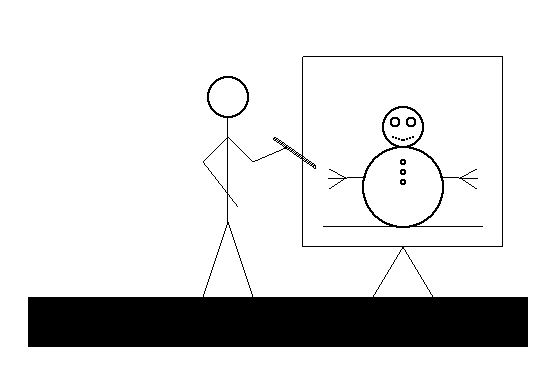
\includegraphics[height=7cm]{Figure/Outputs/OP.png}
\end{figure}

\bigskip\bigskip
\hrule

\end{document}